\chapter{Campos cuánticos locales y ecuación de Dirac unidimensional}

Ya hemos conocido los campos cuánticos a través de sus cuantos, sus operadores de creación y aniquilación, y el Hamiltoniano más sencillo para partículas no relativistas. Ahora pondremos en funcionamiento ese formalismo. Primero veremos, en lugar de limitarnos a afirmarlo, cómo un Hamiltoniano espacialmente local conserva el momento. Después dejaremos que los productos de campos describan dispersión y desintegración, y observaremos cómo la acción repetida del Hamiltoniano genera los primeros elementos de la teoría de perturbaciones diagramática. Solo entonces abordaremos el problema de los fermiones que habíamos anunciado. La forma más sencilla de empezar no es todavía con un campo fermiónico, sino con la ecuación de Dirac unidimensional.

\section{De nuevo, el Hamiltoniano de campo}

Escribamos el Hamiltoniano para una especie de partículas no relativistas como
\begin{equation}
H_0=\int dx\,
\psi^\dagger(x)
\left[-\frac{\partial_x^2}{2m}+V(x)\right]
\psi(x).
\label{eq:l9-nonrel-hamiltonian}
\end{equation}
La notación parece unidimensional, pero nada en el argumento inicial depende de esa restricción: en tres dimensiones, \(x\) puede representar el vector \(\mathbf{x}\), \(dx\) puede representar \(d^3x\) y \(-\partial_x^2\) puede representar \(-\nabla^2\).

El operador \(\psi^\dagger(x)\) crea una partícula en \(x\), mientras que \(\psi(x)\) aniquila una en ese punto. Su producto normalmente ordenado
\begin{equation}
n(x)=\psi^\dagger(x)\psi(x)
\end{equation}
es la densidad local de partículas. Por tanto, el término de potencial es
\begin{equation}
H_V=\int dx\,V(x)n(x).
\end{equation}
exactamente lo que escribiríamos para un gas clásico: contar las partículas cerca de \(x\), asignar a cada una la energía potencial \(V(x)\) y sumarlas en todo el espacio. En esta etapa, las partículas no interactúan entre sí. Pueden responder a un potencial externo aplicado, pero, por lo demás, el Hamiltoniano es una suma de energías independientes de una partícula.

Conviene simplificar y luego volver sobre nuestros pasos. Supongamos que el potencial es constante, \(V(x)=V_0\). Un potencial constante no ejerce fuerza, pero su significado como operador es transparente:
\begin{equation}
\begin{aligned}
H_V&=V_0\int dx\,\psi^\dagger(x)\psi(x)=V_0N,\\
N&=\int dx\,n(x).
\end{aligned}
\end{equation}
Asigna a cada partícula la misma energía aditiva. Para conservar la energía en reposo en una descripción no relativista, elijamos \(V_0=mc^2\). El término cuenta entonces una energía en reposo por partícula. Conservamos esta constante, por lo demás anodina, porque preserva la invariancia traslacional y hace visible la operación de contar partículas.

\section{El Hamiltoniano como regla de actualización}

¿Qué significa decir que se conserva el momento? Debemos formular la respuesta en términos de lo que hace el Hamiltoniano. Para no usar \(\psi\) a la vez para un operador de campo, una función de onda de una partícula y un estado de muchos cuerpos, llamemos \(\lvert\Phi(t)\rangle\) al estado de muchos cuerpos. Durante un intervalo breve \(\epsilon\),
\begin{equation}
\lvert\Phi(t+\epsilon)\rangle
=\left(1-i\epsilon H+O(\epsilon^2)\right)
\lvert\Phi(t)\rangle,
\label{eq:l9-short-update}
\end{equation}
donde \(\hbar=1\). El primer término es el estado sin cambios; la primera corrección la genera \(H\). Iterar esta actualización da la ecuación de Schr\"odinger.

La conservación del momento adquiere ahora un significado concreto. Si el estado inicial tiene un momento total definido \(P\), entonces \(H\lvert\Phi\rangle\) debe tener ese mismo momento total. Otras propiedades pueden cambiar y las partículas individuales pueden intercambiar momento, pero el Hamiltoniano no puede llevar el estado a un sector con un \(P\) total distinto. Podemos comprobarlo directamente reescribiendo el Hamiltoniano en la base de momentos.

\section{La integral espacial como delta de Dirac en el momento}

Elijamos la convención de Fourier
\begin{align}
\psi(x)&=\int\frac{dp}{\sqrt{2\pi}}\,a(p)e^{ipx},\\
\psi^\dagger(x)&=\int\frac{dq}{\sqrt{2\pi}}\,a^\dagger(q)e^{-iqx}.
\label{eq:l9-field-fourier}
\end{align}
El operador \(a(p)\) aniquila una partícula de momento \(p\).
El operador \(a^\dagger(q)\) crea una partícula de momento \(q\). Es esencial usar letras distintas: los dos momentos se integran de forma independiente hasta que la integral espacial los relaciona.

Empecemos por el término de número:
\begin{align}
N
&=\int dx\,\psi^\dagger(x)\psi(x)\\
&=\int\frac{dp\,dq}{2\pi}\,
a^\dagger(q)a(p)
\int dx\,e^{i(p-q)x}.
\end{align}
La integral restante es
\begin{equation}
\int dx\,e^{i(p-q)x}=2\pi\delta(p-q).
\end{equation}
Para \(p\ne q\), la fase oscila y sus contribuciones positivas y negativas se cancelan. Para \(p=q\), no oscila en absoluto. La distribución delta de Dirac es el objeto preciso que reúne ambos hechos. Por consiguiente,
\begin{align}
N
&=\int dp\,dq\,a^\dagger(q)a(p)\delta(p-q)\\
&=\int dp\,a^\dagger(p)a(p).
\label{eq:l9-number-momentum}
\end{align}
El operador elimina una partícula de momento \(p\) y vuelve a crear una con exactamente el mismo momento. El elemento decisivo fue la integral sobre \(x\): produjo la delta que impone la igualdad entre el momento entrante y el saliente.

\begin{classroomqa}
\lecturetimestamp{00:17:02}
\audiencequestion{¿Qué ocurre con el infinito que aparece cuando \(p=q\)?}
\lecturerresponse{Una delta no se utiliza evaluando su altura. Es una distribución definida mediante integración: \(\int dk\,\delta(k)f(k)=f(0)\). La expresión ``infinitamente alta e infinitamente estrecha'' solo nos recuerda que su peso integrado es uno. Aquí nos indica que fijemos \(p-q=0\), y no queda ningún resultado infinito.}
\end{classroomqa}

El mismo mecanismo funciona para un monomio local mucho más general. Supongamos que un término contiene varios campos de aniquilación y varios campos de creación, quizá de especies distintas, pero todos evaluados en un mismo punto e integrados sobre ese punto:
\begin{equation}
\int dx\,
\prod_{r=1}^{n} \psi_{i_r}^\dagger(x)
\prod_{s=1}^{m} \psi_{j_s}(x).
\end{equation}
Sean \(p_s\) los momentos de las partículas aniquiladas y \(q_r\) los de las creadas. El desarrollo de Fourier produce
\begin{equation}
\int dx\,
e^{i(\sum_s p_s-\sum_r q_r)x}
=2\pi\,
\delta\!\left(\sum_s p_s-\sum_r q_r\right).
\label{eq:l9-total-momentum-delta}
\end{equation}
El resultado no empareja \(p_1\) con \(q_1\), \(p_2\) con \(q_2\), y así sucesivamente. Solo impone que
\begin{equation}
\sum_{\mathrm{annihilated}}p
=
\sum_{\mathrm{created}}q.
\end{equation}
Esa es precisamente la regla que debe cumplir una interacción: los momentos individuales pueden cambiar, pero el momento total se conserva. La afirmación más profunda es la invariancia traslacional. Una densidad local integrada con el mismo peso en todos los puntos no tiene un origen preferido, y su transformada de Fourier lleva la delta correspondiente que conserva el momento.

\begin{classroomqa}
\lecturetimestamp{00:23:04}
\audiencequestion{¿El término propuesto del Hamiltoniano es realmente un producto de todos esos operadores de campo? ¿Por qué escribiríamos un producto así?}
\lecturerresponse{Sí. El producto especifica qué partículas se eliminan y cuáles se crean en un mismo punto. Su motivación física provendrá de los procesos de dispersión o desintegración observados; primero establecemos el argumento sobre el momento para poder identificar esas interacciones de inmediato.}
\end{classroomqa}

\section{La energía cinética en el espacio de momentos y de posiciones}

Apliquemos ahora el mismo formalismo al término con derivadas. La derivada actúa sobre la onda plana:
\begin{equation}
-\partial_x^2 e^{ipx}=p^2e^{ipx}.
\end{equation}
Por tanto,
\begin{align}
H_{\mathrm{kin}}
&=\int dx\,\psi^\dagger(x)
\left(-\frac{\partial_x^2}{2m}\right)\psi(x)\\
&=\int dp\,\frac{p^2}{2m}\,a^\dagger(p)a(p).
\label{eq:l9-kinetic-momentum}
\end{align}
De nuevo, la integral espacial impone que el momento entrante y el saliente sean iguales. El nuevo factor \(p^2/2m\) simplemente pondera el número de partículas de cada modo de momento por la energía cinética de ese modo.

\begin{classroomqa}
\lecturetimestamp{00:24:46}
\audiencequestion{¿Al derivar dos veces la onda plana no debería aparecer un signo menos?}
\lecturerresponse{Sí, \(\partial_x^2e^{ipx}=-p^2e^{ipx}\). El Hamiltoniano ya contiene el signo menos compensatorio, de modo que \(-\partial_x^2\) tiene el autovalor positivo \(p^2\).}
\end{classroomqa}

\begin{classroomqa}
\lecturetimestamp{00:27:20}
\audiencequestion{¿Solo se conserva la energía cinética cuando el potencial es constante?}
\lecturerresponse{Sí. Si no hay un potencial dependiente de la posición, no hay fuerza y la energía cinética se conserva por separado. En un potencial externo no constante, la energía cinética y la potencial pueden intercambiarse, mientras que el Hamiltoniano total se conserva si no depende explícitamente del tiempo.}
\end{classroomqa}

\begin{classroomqa}
\lecturetimestamp{00:27:42}
\audiencequestion{¿Qué función cumple \(\psi^\dagger\psi\) en el Hamiltoniano cinético en el espacio de momentos?}
\lecturerresponse{Es el operador de número. El producto de modos \(a^\dagger(p)a(p)\) cuenta las partículas de momento \(p\), y el factor \(p^2/2m\) asigna a cada una la energía cinética correspondiente.}
\end{classroomqa}

Hay otra forma de ver que la energía es positiva. Una integración por partes y el descarte del término de frontera dan
\begin{align}
\int dx\,\psi^\dagger(-\partial_x^2)\psi
&=\int dx\,(\partial_x\psi^\dagger)(\partial_x\psi).
\label{eq:l9-positive-kinetic}
\end{align}
Para campos que se anulan de manera adecuada en el infinito, o con condiciones de contorno periódicas, la contribución de frontera es cero. El resultado tiene la forma de un cuadrado de módulo y es no negativo. También muestra un patrón común en la teoría de campos: la energía contiene cuadrados de derivadas espaciales de los campos.

\section{Una interacción local de contacto}

Démosles ahora a los productos de campos una función física. Consideremos dos especies, a las que llamaremos electrón y protón solo para que la imagen resulte familiar. Por ahora son deliberadamente ficticias: ambas se describen mediante operadores bosónicos y se omite su verdadera interacción de Coulomb. Su Hamiltoniano libre es
\begin{equation}
H_0=\int dx\left[
\psi_e^\dagger\left(-\frac{\partial_x^2}{2m_e}\right)\psi_e
+
\psi_p^\dagger\left(-\frac{\partial_x^2}{2m_p}\right)\psi_p
\right].
\end{equation}
Añadamos la interacción modelo
\begin{equation}
H_{\mathrm{contact}}
=g\int dx\,
\psi_e^\dagger(x)\psi_p^\dagger(x)
\psi_e(x)\psi_p(x).
\label{eq:l9-contact}
\end{equation}
Leámosla de derecha a izquierda. Busca un electrón y un protón en el mismo punto \(x\), los aniquila y vuelve a crear ambos en ese punto. Si las dos partículas no están juntas, este término local da cero. Si sus líneas de universo se encuentran, puede cambiar sus momentos individuales y conservar el momento total. Así, actúa como un potencial de dispersión idealizado de alcance nulo.

\begin{figure}[htbp]
\centering
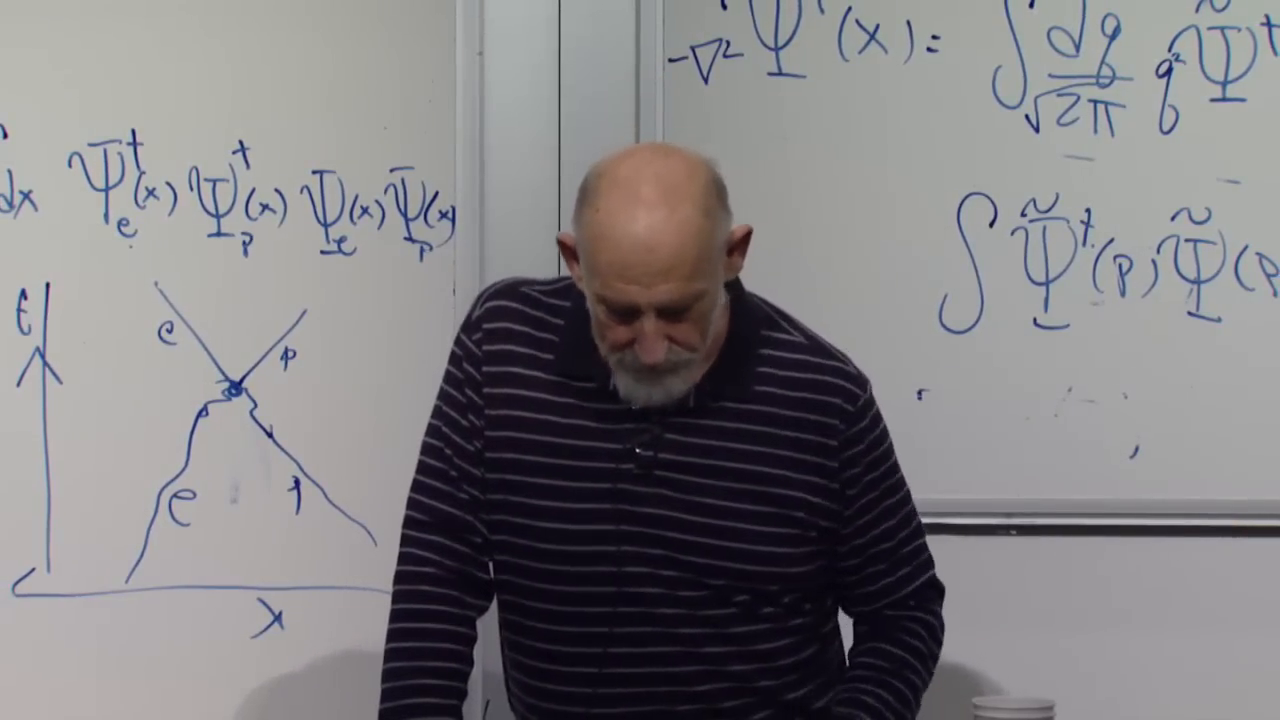
\includegraphics[width=0.94\linewidth]{lecture_09_frame_02.png}
\caption{La interacción de contacto en la pizarra. Los cuatro operadores de campo locales aparecen sobre el esquema espaciotemporal; el punto de encuentro es el único lugar donde actúa la interacción idealizada.}
\lectureframe{00:35:36}
\end{figure}

\begin{figure}[htbp]
\centering
\begin{tikzpicture}[x=1.2cm,y=1.0cm,>=Latex]
\draw[->] (-3.0,0) -- (3.0,0) node[right] {$x$};
\draw[->] (0,-0.2) -- (0,4.2) node[above] {$t$};
\coordinate (v) at (0,2.0);
\fill (v) circle (1.8pt);
\draw[thick,->] (-2.2,0.4) -- (v);
\draw[thick,->] (2.0,0.4) -- (v);
\draw[thick,->] (v) -- (-1.6,3.7);
\draw[thick,->] (v) -- (2.2,3.7);
\node[left] at (-1.65,0.7) {$e$};
\node[right] at (1.55,0.7) {$p$};
\node[left] at (-1.15,3.3) {$e$};
\node[right] at (1.65,3.3) {$p$};
\node[right] at (0.12,2.05) {$g$};
\end{tikzpicture}
\caption{Reconstrucción limpia de la imagen de dispersión local. El vértice es una abreviatura del operador de la ecuación~\eqref{eq:l9-contact}, no una ley clásica de colisión.}
\end{figure}

Los electrones y protones reales interactúan a distancia mediante el potencial de Coulomb. El modelo de contacto es solo un primer paso, válido para distancias cortas: si los experimentos mostraran que dos especies se dispersan únicamente cuando se solapan, incluiríamos en el Hamiltoniano un término del tipo de la ecuación~\eqref{eq:l9-contact}.

\begin{classroomqa}
\lecturetimestamp{00:35:40}
\audiencequestion{¿Por qué forma parte del Hamiltoniano este operador de dispersión si la energía no cambia?}
\lecturerresponse{El Hamiltoniano es tanto el operador de energía como el generador de cambios en el estado. La energía potencial entre las dos partículas produce dispersión durante la evolución temporal. Que se conserve la energía total no significa que el estado o los momentos individuales de las partículas permanezcan inalterados.}
\end{classroomqa}

Esto da una regla práctica. Primero, averigüemos mediante experimentos qué procesos locales pueden experimentar las partículas. Después, codifiquemos esos procesos en el operador que actualiza el estado. Los productos de campos no son álgebra decorativa: sus factores con daga y sin daga especifican qué especies aparecen y desaparecen.

\section{Desintegración, proceso inverso y hermiticidad}

Supongamos que en una cámara de burbujas se observa una traza de la especie \(A\) que termina en un punto del que emergen trazas de \(B\) y \(C\). El proceso local es
\begin{equation}
A\longrightarrow B+C.
\end{equation}
El operador que lo realiza es
\begin{equation}
V=g\int dx\,
\psi_B^\dagger(x)\psi_C^\dagger(x)\psi_A(x).
\label{eq:l9-decay-half}
\end{equation}
El campo de aniquilación elimina \(A\); los dos campos de creación producen \(B\) y \(C\) en el mismo punto. Integrar con el mismo peso sobre cada \(x\) expresa la invariancia traslacional espacial y proporciona inmediatamente
\begin{equation}
p_A=p_B+p_C.
\end{equation}

Un Hamiltoniano debe ser hermítico. Esto es lo que hace que \(e^{-itH}\) sea unitario y preserve la probabilidad total. La ecuación~\eqref{eq:l9-decay-half} no es hermítica por sí sola, así que debemos añadir su adjunto:
\begin{equation}
H_{\mathrm{int}}
=\int dx\left[
g\,\psi_B^\dagger\psi_C^\dagger\psi_A
+g^*\,\psi_A^\dagger\psi_C\psi_B
\right](x).
\label{eq:l9-hermitian-vertex}
\end{equation}
Para un acoplamiento real \(g\), los dos coeficientes son iguales. La conjugación hermítica invierte el orden de los operadores, además de intercambiar los campos con daga y sin daga. En este modelo bosónico de juguete, los campos de especies distintas conmutan, por lo que esa inversión no introduce complicaciones adicionales.

El segundo término realiza el proceso inverso,
\begin{equation}
B+C\longrightarrow A.
\end{equation}
Así, un Hamiltoniano cerrado y unitario que permite la desintegración también contiene la amplitud de recombinación. Esto no garantiza que ambas direcciones ocurran para cualquier conjunto de momentos externos: las leyes de conservación de la energía y otras pueden impedir que una de ellas sea cinemáticamente accesible. Significa que tanto el operador como su adjunto forman parte de la dinámica.

\begin{classroomqa}
\lecturetimestamp{00:42:48}
\audiencequestion{¿Puede haber una excepción a la regla de que también se permite el proceso inverso?}
\lecturerresponse{No en el marco de un Hamiltoniano hermítico de un sistema cerrado: se requiere la interacción adjunta. Una reacción inversa concreta aún puede verse impedida por la cinemática o por otro número cuántico conservado, pero el elemento de matriz conjugado está presente.}
\end{classroomqa}

El número \(g\) es la constante de acoplamiento. Si \(g\) es pequeño, las partículas que se encuentran interactúan débilmente; si es grande, la amplitud de transición es mayor. Por lo general, los acoplamientos son parámetros medidos experimentalmente, aunque las simetrías pueden relacionar varios acoplamientos que a primera vista parecen distintos.

La misma estructura permite describir reacciones más elaboradas. En la desintegración beta,
\begin{equation}
n\longrightarrow p+e^-+\bar\nu_e,
\end{equation}
un término local esquemático contiene cuatro campos: uno aniquila el neutrón y tres crean el protón, el electrón y el antineutrino electrónico, junto con el proceso conjugado hermítico. Esto basta para ver cómo un pequeño conjunto de monomios de operadores empieza a definir una teoría cuántica de campos.

\section{Por qué importa el cuadrado del Hamiltoniano}

La fórmula para tiempos cortos \eqref{eq:l9-short-update} solo conservaba los términos de primer orden en \(\epsilon\). El desarrollo completo es
\begin{equation}
e^{-i\epsilon H}
=1-i\epsilon H-\frac{\epsilon^2}{2}H^2
+\frac{i\epsilon^3}{3!}H^3+\cdots.
\label{eq:l9-exponential}
\end{equation}
A segundo orden, el Hamiltoniano actúa dos veces. Este es el origen algebraico de las primeras representaciones de procesos compuestos.

Para el vértice \(A\leftrightarrow B+C\), una acción puede combinar \(B+C\) para formar \(A\), y una segunda puede descomponer ese \(A\) de nuevo en \(B+C\):
\begin{equation}
B+C\longrightarrow A\longrightarrow B+C.
\label{eq:l9-bc-scattering}
\end{equation}
La contribución neta es una amplitud de dispersión \(B+C\to B+C\). El estado intermedio \(A\) no es un suceso observado adicional; indica el estado sobre el que se suma entre dos acciones de la interacción.

\begin{classroomqa}
\lecturetimestamp{00:49:54}
\audiencequestion{¿El campo de \(C\) de la expresión escrita de segundo orden debería llevar una daga?}
\lecturerresponse{Sí, el orden de los operadores debe corresponder a la secuencia indicada. El primer vértice aniquila \(B\) y \(C\), y crea \(A\); el segundo aniquila \(A\) y vuelve a crear \(B\) y \(C\). Escribir correctamente las dagas correspondientes restablece esa interpretación.}
\end{classroomqa}

\begin{figure}[htbp]
\centering
\includegraphics[width=0.94\linewidth]{lecture_09_frame_05.png}
\caption{Las dos orientaciones del vértice elemental \(A\leftrightarrow B+C\) en la pizarra. Colocarlas una junto a otra es la representación visual abreviada del proceso de segundo orden de la ecuación~\eqref{eq:l9-bc-scattering}.}
\lectureframe{00:48:56}
\end{figure}

Añadamos ahora un \(B\) espectador. Una acción permite que \(A\) emita \(C\) y se convierta en \(B\); una acción posterior permite que ese \(C\) se combine con el \(B\) original para formar \(A\). Las partículas externas vuelven a ser \(A+B\), pero sus momentos pueden cambiar. Describimos esto como dispersión de \(A\) y \(B\) mediante el intercambio de \(C\).

\begin{figure}[htbp]
\centering
\includegraphics[width=0.94\linewidth]{lecture_09_frame_06.png}
\caption{La construcción de intercambio en la pizarra. El diagrama de la derecha une dos vértices elementales mediante una línea interna de \(C\), mientras las partículas externas \(A\) y \(B\) se dispersan.}
\lectureframe{00:51:22}
\end{figure}

\begin{figure}[htbp]
\centering
\begin{tikzpicture}[x=1.1cm,y=1cm,>=Latex]
\draw[->] (-3.7,-0.2) -- (-3.7,4.2) node[above] {$t$};
\coordinate (v1) at (-0.9,1.25);
\coordinate (v2) at (0.9,2.95);
\fill (v1) circle (1.7pt);
\fill (v2) circle (1.7pt);
\draw[thick,->] (-2.6,0.2) -- (v1) node[midway,below left] {$A$};
\draw[thick,->] (2.6,0.2) -- (v2) node[midway,below right] {$B$};
\draw[thick,->] (v1) -- (-2.4,4.0) node[midway,left] {$B$};
\draw[thick,->] (v2) -- (2.5,4.0) node[midway,right] {$A$};
\draw[thick,->,dashed] (v1) -- (v2) node[midway,above left] {$C$};
\node[below] at (0,-0.05) {$A+B\rightarrow A+B$};
\end{tikzpicture}
\caption{Reconstrucción limpia del intercambio de \(C\). Cada punto aporta un factor de \(g\), por lo que este término de segundo orden es proporcional a \(g^2\).}
\end{figure}

Cada punto de interacción local se denomina vértice. Cada vértice aporta un factor de su acoplamiento, así que una contribución con dos vértices lleva \(g^2\), una con tres vértices lleva \(g^3\), y así sucesivamente. Por tanto, un solo término del Hamiltoniano correlaciona una gran familia de reacciones. Esta economía es una de las razones por las que la teoría cuántica de campos es tan potente: un pequeño número de interacciones locales organiza una enorme cantidad de datos de dispersión.

\begin{classroomqa}
\lecturetimestamp{00:53:14}
\audiencequestion{¿Cómo se llama el proceso \(A\to B+C\to A\)?}
\lecturerresponse{Es una contribución de autoenergía. Un \(A\) medido no es simplemente el estado de base desnudo de una partícula; el estado interactuante también tiene una amplitud para componentes cercanas \(B+C\). La dispersión desde ese estado puede revelar su estructura vestida.}
\end{classroomqa}

La electrodinámica cuántica ofrece el ejemplo conocido. Un vértice local electrón--fotón puede aniquilar un electrón, volver a crear un electrón y crear un fotón. A segundo orden, el electrón puede emitir y reabsorber un fotón. Es tentador narrarlo como una pequeña película, pero su significado preciso es el de un término en el desarrollo perturbativo. El electrón físico es un estado vestido con componentes que contienen fotones.

La estimación didáctica de que esta componente es ``aproximadamente un uno por ciento'' transmite la escala que fija la constante de estructura fina, \(\alpha_{\mathrm{em}}\simeq 1/137\). La probabilidad precisa de una componente del espacio de Fock con fotones depende de la resolución energética y de cómo se defina el estado interactuante; no es una propiedad universal de un electrón aislado que valga un uno por ciento. La afirmación robusta es que la interacción modifica la estructura medible del electrón.

\section{Qué representa un diagrama y qué no}

Los diagramas son una abreviatura de cálculo para las potencias del Hamiltoniano de interacción. No son historias clásicas fiables en las que una partícula realiza definitivamente un suceso y luego otro. Mirar en el interior para decidir qué alternativa intermedia ``ocurrió realmente'' cambia el experimento y destruye la suma coherente, igual que en la interferencia cuántica ordinaria.

\begin{classroomqa}
\lecturetimestamp{00:56:52}
\audiencequestion{¿Se conservan tanto la energía como el momento en el primer vértice?}
\lecturerresponse{En la construcción hamiltoniana a tiempo igual que hemos realizado aquí, la integral espacial produce inmediatamente una delta de momento. En esa inserción aislada aún no se ha realizado ninguna integral temporal que produzca una delta de energía. La amplitud de dispersión completa, invariante bajo traslaciones temporales, conserva la energía total, mientras que las líneas intermedias no tienen por qué satisfacer la relación de capa de masa de las partículas observadas. En el lenguaje de los diagramas covariantes, el cuadrimomento se conserva en cada vértice, pero las partículas internas pueden estar fuera de la capa de masa.}
\end{classroomqa}

La aparente falta de energía en una imagen ingenua del vértice es otra advertencia de que no se debe descartar la energía de interacción. El Hamiltoniano total es más que la suma de las energías de las partículas libres. Si surge alguna confusión, volvamos a la ecuación~\eqref{eq:l9-exponential}: la imagen representa un término del desarrollo de la evolución temporal unitaria. El formalismo completo de los diagramas de Feynman proporciona ordenamiento temporal sistemático, propagadores, integrales y factores de simetría, pero la física básica empieza aquí.

Una pregunta más extensa lleva a interpretar el diagrama de forma demasiado literal al comparar el fotón emitido con el campo eléctrico que rodea a un electrón que se mueve lentamente.

\begin{classroomqa}
\lecturetimestamp{00:58:26}
\audiencequestion{¿El campo eléctrico del electrón a distancia lo producen literalmente fotones radiados? ¿Cómo encaja esto con la interferencia y el efecto Aharon--Bohm?}
\lecturerresponse{Un campo estático o de inducción no es un flujo de fotones reales radiados. La electrodinámica cuántica describe tanto la radiación como el vestido electromagnético del electrón mediante el mismo campo, pero los estados cuánticos y la cinemática correspondientes son distintos. Para un electrón ultrarrelativista, algunos componentes del campo pueden comportarse útilmente como un flujo de fotones casi reales; para un electrón lento, una trayectoria literal de fotones es un modelo incorrecto. La interferencia de doble rendija y el efecto Aharon--Bohm también son fenómenos de campo no clásicos, pero no convierten este diagrama de autoenergía en una película mecánica.}
\end{classroomqa}

\begin{classroomqa}
\lecturetimestamp{01:01:28}
\audiencequestion{¿Por qué falla exactamente un modelo clásico del diagrama?}
\lecturerresponse{Porque el cálculo suma coherentemente las amplitudes de todas las alternativas intermedias permitidas. La experiencia hace intuitivas estas imágenes, pero su contenido literal nunca va más allá del desarrollo de operadores que las define. Son una forma compacta de calcular \(H^2,H^3,\ldots\), no un registro de sucesos intermedios observados.}
\end{classroomqa}

\begin{classroomqa}
\lecturetimestamp{01:03:04}
\audiencequestion{¿Puede surgir la interacción de Coulomb ordinaria como límite clásico del intercambio de fotones?}
\lecturerresponse{Sí. Al evaluar la amplitud pertinente mediada por fotones y tomar el límite estático no relativista se obtiene el potencial de Coulomb. La derivación es más técnica que el esquema de operadores que presentamos aquí, y aun así no debe interpretarse como si un fotón saltara literalmente entre dos partículas clásicas.}
\end{classroomqa}

\begin{classroomqa}
\lecturetimestamp{01:03:44}
\audiencequestion{¿Se calculan las constantes de acoplamiento a partir de los productos de campos?}
\lecturerresponse{Por lo general, sus valores numéricos se introducen a partir de datos experimentales. Las simetrías pueden restringirlos o relacionar acoplamientos que de otro modo serían independientes. Cuando una relación así predice las intensidades relativas de reacciones distintas y el experimento la confirma, esa concordancia aporta información especialmente valiosa.}
\end{classroomqa}

\begin{classroomqa}
\lecturetimestamp{01:04:48}
\audiencequestion{¿Qué papel tiene una simetría accidental frente a una simetría gauge?}
\lecturerresponse{La simetría gauge restringe directamente la estructura permitida y las relaciones entre acoplamientos. Una simetría accidental no se impone a nivel fundamental, sino que emerge porque todas las interacciones permitidas de orden inferior la respetan por casualidad. Aun así, puede tener consecuencias importantes, aunque su origen y robustez difieren de los de una simetría gauge.}
\end{classroomqa}

Por ahora, basta con la teoría de campos no relativista. Habíamos prometido hablar de fermiones. En vez de cuantizarlos en segunda cuantización de inmediato, primero entenderemos la ecuación relativista de una partícula que deben satisfacer sus operadores de campo.

\section{Por qué el electrón requiere la relatividad}

Empecemos con una dimensión espacial. No es una restricción realista, pero elimina la complejidad geométrica del espín tridimensional y conserva el álgebra esencial. El electrón es lo bastante ligero como para que la relatividad importe incluso en los átomos. En el hidrógeno, su velocidad característica es del orden de
\begin{equation}
v\sim\alpha_{\mathrm{em}}c\approx 0.007c,
\end{equation}
aproximadamente un uno por ciento de la velocidad de la luz. Para los electrones internos de un átomo pesado, la escala aproximada pasa a ser \(v\sim Z\alpha_{\mathrm{em}}c\), por lo que las correcciones relativistas pueden ser sustanciales. Tanto si la motivación decisiva fue la curiosidad histórica como si fue la precisión atómica, una ecuación de tipo Schr\"odinger relativista es físicamente necesaria.

La receta habitual de cuantización parte de la relación clásica entre energía y momento. En el régimen no relativista,
\begin{equation}
E=\frac{p^2}{2m},
\end{equation}
y las sustituciones
\begin{equation}
E\mapsto i\partial_t,
\qquad
p\mapsto-i\partial_x
\end{equation}
producen
\begin{equation}
i\partial_t\varphi(x,t)
=-\frac{1}{2m}\partial_x^2\varphi(x,t).
\end{equation}

En cambio, la relatividad da, con \(c=1\),
\begin{equation}
E^2=p^2+m^2.
\label{eq:l9-rel-dispersion}
\end{equation}

\begin{figure}[htbp]
\centering
\includegraphics[width=0.94\linewidth]{lecture_09_frame_07.png}
\caption{El paso en la pizarra de \(E=p^2/2m\) a la relación relativista \(E^2=p^2+m^2\), con \(c=1\).}
\lectureframe{01:10:30}
\end{figure}

Aplicar las sustituciones a la relación al cuadrado da
\begin{equation}
-\partial_t^2\varphi
=\left(-\partial_x^2+m^2\right)\varphi,
\label{eq:l9-klein-gordon}
\end{equation}
o, de manera equivalente,
\begin{equation}
\left(\partial_t^2-\partial_x^2+m^2\right)\varphi=0.
\end{equation}
Esta es la ecuación de Klein--Gordon. Es una ecuación relativista de campo perfectamente válida, sobre todo para campos de espín cero. Pero la ecuación buscada para el electrón debe ser de primer orden en el tiempo,
\begin{equation}
i\partial_t\Psi=H\Psi,
\end{equation}
para que \(H\) mismo, y no solo \(H^2\), genere la evolución.

Formalmente, se podría elegir
\begin{equation}
H=\sqrt{-\partial_x^2+m^2}.
\end{equation}
La raíz cuadrada se define limpiamente en el espacio de momentos, donde multiplica por \(\sqrt{p^2+m^2}\), pero en el espacio de posiciones es un operador pseudodiferencial no local. Tiene sentido técnico, pero resulta poco adecuada desde el punto de vista estético para la ecuación local que buscamos. Empecemos, pues, de nuevo.

\section{Una onda sin masa que se mueve hacia la derecha}

Consideremos primero una partícula sin masa que se mueve hacia la derecha. Su energía positiva y su momento satisfacen
\begin{equation}
E=p
\qquad (c=1).
\end{equation}
La cuantización da
\begin{equation}
i\partial_t\psi=-i\partial_x\psi,
\end{equation}
o bien
\begin{equation}
(\partial_t+\partial_x)\psi=0.
\label{eq:l9-right-mover}
\end{equation}
Toda solución tiene la forma
\begin{equation}
\psi(x,t)=f(x-t).
\end{equation}
El perfil es rígido y se mueve hacia la derecha a la velocidad de la luz.

De inmediato aparecen dos dificultades. Primero, si se permite que la ecuación~\eqref{eq:l9-right-mover} actúe sobre modos de Fourier arbitrarios, un momento negativo tiene energía \(E=p<0\), de modo que el Hamiltoniano no está acotado inferiormente. Restringirlo a mano a \(p>0\) conservaría solo las ondas que se mueven hacia la derecha y todavía no nos daría la teoría del electrón que buscamos. Segundo, la ecuación solo permite propagación en un sentido: no contiene un electrón ordinario que se mueva hacia la izquierda. Resolveremos primero el problema de las direcciones izquierda y derecha y dejaremos expuestas las energías negativas.

\section{Dos componentes y la matriz alfa}

Introduzcamos dos amplitudes,
\begin{equation}
\Psi(x,t)=
\begin{pmatrix}
\psi_1(x,t)\\[3pt]
\psi_2(x,t)
\end{pmatrix},
\end{equation}
donde \(\psi_1\) se mueve hacia la derecha y \(\psi_2\) hacia la izquierda en el límite sin masa:
\begin{align}
(\partial_t+\partial_x)\psi_1&=0,
&
(\partial_t-\partial_x)\psi_2&=0.
\end{align}
La mecánica cuántica también permite superposiciones arbitrarias de ambas. Por tanto, una partícula puede tener amplitudes correspondientes a las dos direcciones, en lugar de llevar una etiqueta clásica elegida de una vez para siempre.

Este grado de libertad adicional de dos valores se parece algebraicamente al espín, pero en una dimensión no es momento angular ordinario. Definamos
\begin{equation}
\alpha=
\begin{pmatrix}
1&0\\
0&-1
\end{pmatrix}
=\sigma_3.
\label{eq:l9-alpha}
\end{equation}
Su vector propio de valor propio \(+1\) selecciona la componente que se propaga hacia la derecha, y el de valor propio \(-1\), la que se propaga hacia la izquierda. En la teoría sin masa, el hamiltoniano es simplemente
\begin{equation}
H=\alpha p,
\end{equation}
y las dos ecuaciones se combinan en
\begin{equation}
i\partial_t\Psi=-i\alpha\partial_x\Psi.
\label{eq:l9-massless-dirac}
\end{equation}

\begin{classroomqa}
\lecturetimestamp{01:22:44}
\audiencequestion{¿Cómo se llama la matriz diagonal que distingue las dos componentes?}
\lecturerresponse{Como matriz de Pauli es \(\sigma_3\), no \(\sigma_1\). En la notación de Dirac para la construcción que estamos desarrollando, la llamamos \(\alpha\). Su álgebra es la conocida álgebra de Pauli, aunque aquí la etiqueta física es la dirección, no el momento angular de espín.}
\end{classroomqa}

\begin{classroomqa}
\lecturetimestamp{01:23:32}
\audiencequestion{¿Adquiere la construcción un significado más geométrico en tres dimensiones, donde la dirección es un vector?}
\lecturerresponse{Sí. El problema tridimensional requiere una matriz para cada dirección espacial y conduce a una estructura de espinores más rica. Aun así, el modelo unidimensional es exacto en su propio ámbito y aísla el álgebra esencial de derecha e izquierda sin esa complejidad adicional.}
\end{classroomqa}

\begin{figure}[htbp]
\centering
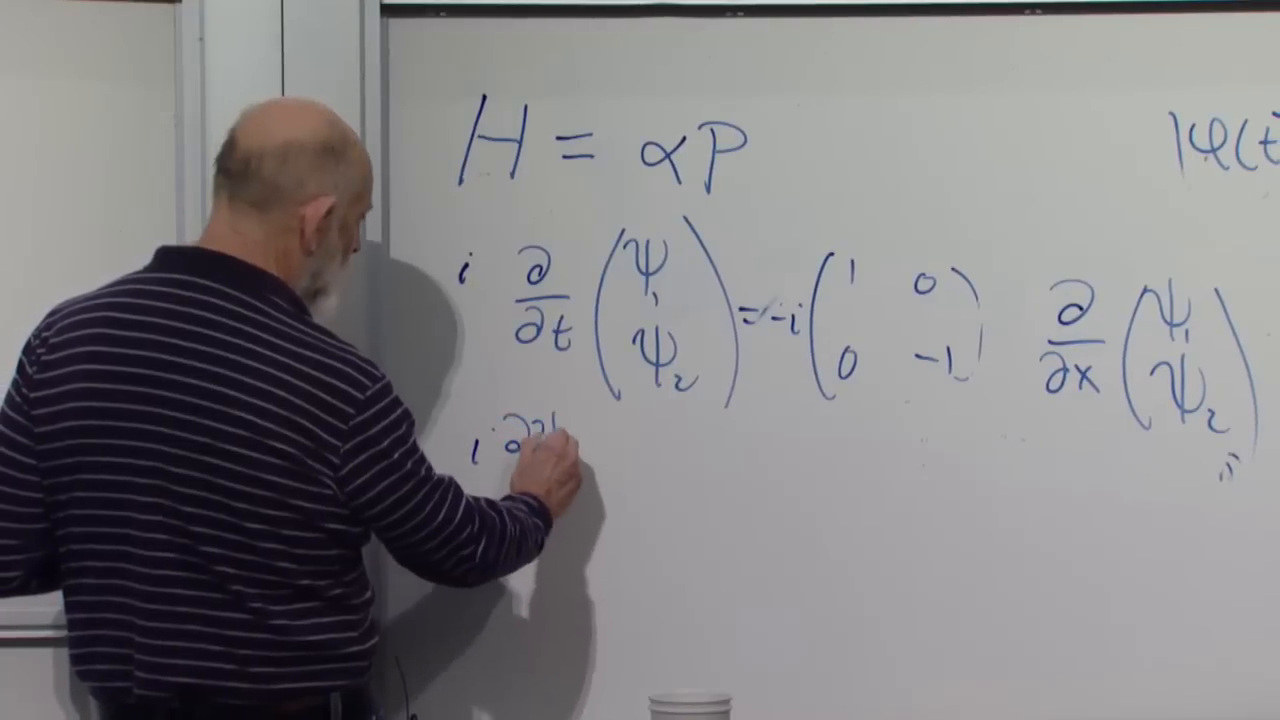
\includegraphics[width=0.94\linewidth]{lecture_09_frame_03.png}
\caption{La ecuación sin masa de dos componentes escrita en la pizarra: \(H=\alpha P\), con la matriz diagonal que asigna propagación en sentidos opuestos a \(\psi_1\) y \(\psi_2\).}
\lectureframe{01:26:00}
\end{figure}

El problema de la propagación en un solo sentido ha desaparecido. El espectro de energías negativas persiste, y hemos descubierto un tercer defecto: las dos componentes siguen siendo sin masa y se propagan a la velocidad de la luz. El siguiente paso debe introducir una energía en reposo y acoplar las dos direcciones.

\section{Añadir masa y descubrir el álgebra de Dirac}

Añadamos el término más general y sencillo proporcional a la masa:
\begin{equation}
H=\alpha p+\beta m,
\label{eq:l9-dirac-hamiltonian}
\end{equation}
donde \(\beta\) actúa solo sobre el índice de las dos componentes. Podría haber sido la identidad u otra matriz; dejaremos que la relación de dispersión relativista decida.

Como \(H^2\) debe ser igual a \(p^2+m^2\), elevemos al cuadrado la Ec.~\eqref{eq:l9-dirac-hamiltonian}:
\begin{align}
H^2
&=(\alpha p+\beta m)^2\\
&=\alpha^2p^2+\beta^2m^2
+(\alpha\beta+\beta\alpha)pm.
\label{eq:l9-square-dirac}
\end{align}
Las matrices conmutan con \(p\) porque actúan en el espacio interno de dos componentes, mientras que \(p\) actúa sobre la función de onda espacial. Para que concuerde con la Ec.~\eqref{eq:l9-rel-dispersion} se requiere
\begin{equation}
\alpha^2=\mathbb{1},
\qquad
\beta^2=\mathbb{1},
\qquad
\{\alpha,\beta\}
=\alpha\beta+\beta\alpha=0.
\label{eq:l9-dirac-algebra}
\end{equation}
La primera condición ya se cumple para \(\alpha=\sigma_3\). Cualquier otra matriz de Pauli anticonmuta con ella y su cuadrado es la identidad. Elijamos
\begin{equation}
\beta=
\begin{pmatrix}
0&1\\
1&0
\end{pmatrix}
=\sigma_1.
\label{eq:l9-beta}
\end{equation}
Elegir \(\sigma_1\) en lugar de \(\sigma_2\) es una convención de base; ambas realizan la misma álgebra tras un cambio unitario de base.

\begin{classroomqa}
\lecturetimestamp{01:33:00}
\audiencequestion{¿Dirac se limitó a reconocer que las matrices de Pauli satisfacen estas condiciones algebraicas?}
\lecturerresponse{La derivación histórica se llevó a cabo directamente en tres dimensiones e introdujo matrices que satisfacían las relaciones requeridas. Una vez escritas las condiciones, el álgebra de Pauli hace inmediata la solución unidimensional: basta elegir dos matrices de Pauli distintas.}
\end{classroomqa}

\begin{classroomqa}
\lecturetimestamp{01:34:24}
\audiencequestion{¿Es esta \(\beta\) el parámetro relativista de velocidad \(v/c\)?}
\lecturerresponse{No. Es una matriz que actúa sobre las componentes del espinor. La letra reutilizada es solo la notación de Dirac; no tiene nada que ver con la magnitud cinemática \(v/c\).}
\end{classroomqa}

En tres dimensiones espaciales, las matrices \(2\times2\) no bastan para formar el conjunto completo de matrices anticomutantes requerido. Dejaremos esa ampliación para más adelante. En una dimensión, las Ecs.~\eqref{eq:l9-alpha} y \eqref{eq:l9-beta} son suficientes.

\section{La ecuación de Dirac unidimensional acoplada}

Al sustituir \(p=-i\partial_x\), obtenemos la ecuación de Dirac unidimensional en forma hamiltoniana:
\begin{equation}
i\partial_t\Psi
=\left(-i\alpha\partial_x+\beta m\right)\Psi.
\label{eq:l9-one-dimensional-dirac}
\end{equation}
Como \(\alpha\) es diagonal, su término derivativo mantiene separadas las dos componentes. Como \(\beta\) es no diagonal, el término de masa las intercambia. Escrita componente a componente,
\begin{align}
i\partial_t\psi_1
&=-i\partial_x\psi_1+m\psi_2,
\label{eq:l9-dirac-component-one}\\
i\partial_t\psi_2
&=+i\partial_x\psi_2+m\psi_1.
\label{eq:l9-dirac-component-two}
\end{align}

\begin{figure}[htbp]
\centering
\includegraphics[width=0.94\linewidth]{lecture_09_frame_08.png}
\caption{Las ecuaciones acopladas para las componentes, escritas en la pizarra. Los signos opuestos de las derivadas codifican la propagación hacia la derecha y hacia la izquierda; el término de masa no diagonal intercambia \(\psi_1\) y \(\psi_2\).}
\lectureframe{01:37:44}
\end{figure}

Las componentes dejan de evolucionar independientemente en cuanto \(m\ne0\). Al elevar al cuadrado la ecuación de primer orden, se recupera el operador de Klein--Gordon en cada componente:
\begin{equation}
\left(\partial_t^2-\partial_x^2+m^2\right)\psi_a=0,
\qquad a=1,2,
\end{equation}
y las ondas planas satisfacen \(E^2=p^2+m^2\). Su velocidad de grupo es
\begin{equation}
v_g=\frac{dE}{dp}=\frac{p}{E},
\end{equation}
y su módulo es menor que uno si la masa no es nula.

La relación entre la masa y la mezcla de las componentes derecha e izquierda no es casual. Una partícula sin masa que se propaga hacia la derecha sigue haciéndolo bajo cualquier transformación de Lorentz propia: ningún observador sublumínico puede adelantarse a la luz e invertir su dirección. Una partícula masiva puede llevarse al reposo y luego observarse desde un sistema de referencia más rápido que se mueve en la misma dirección, en el que su velocidad parece invertirse. Por tanto, una teoría relativista con masa no puede mantener los sectores derecho e izquierdo permanentemente aislados. El término de masa no diagonal proporciona precisamente el acoplamiento requerido.

\begin{classroomqa}
\lecturetimestamp{01:40:01}
\audiencequestion{¿El intercambio entre las dos componentes es una oscilación quiral?}
\lecturerresponse{En esta base unidimensional, \(\alpha\) distingue las dos direcciones quirales sin masa. El término de masa es no diagonal y las mezcla, de modo que la quiralidad deja de conservarse. En ese sentido, el término de masa es el origen de la oscilación quiral.}
\end{classroomqa}

\begin{classroomqa}
\lecturetimestamp{01:40:46}
\audiencequestion{¿Por qué una ecuación para fermiones tendría que ser la raíz cuadrada de una ecuación para bosones?}
\lecturerresponse{No debe entenderse de ese modo. La relación de dispersión \(E^2=p^2+m^2\) se aplica a toda partícula relativista libre, independientemente de sus estadísticas. El operador de Dirac resulta proporcionar una factorización matricial del operador de Klein--Gordon, pero esa relación algebraica no deriva los fermiones de los bosones.}
\end{classroomqa}

\begin{classroomqa}
\lecturetimestamp{01:41:31}
\audiencequestion{¿Puede reducirse la ecuación a una factorización escalar sencilla en factores separados de propagación hacia la derecha y hacia la izquierda?}
\lecturerresponse{Solo en el límite sin masa se desacoplan las dos ecuaciones quirales en factores escalares independientes. Para \(m\ne0\), la factorización útil es matricial: las matrices anticomutantes \(\alpha\) y \(\beta\) son las que eliminan el término cruzado no deseado.}
\end{classroomqa}

\begin{classroomqa}
\lecturetimestamp{01:42:04}
\audiencequestion{¿Constituyen ya estas dos ecuaciones acopladas la ecuación de Dirac?}
\lecturerresponse{Sí. Juntas forman la ecuación de Dirac en una dimensión espacial, escrita de manera equivalente en la forma compacta de la Ec.~\eqref{eq:l9-one-dimensional-dirac}. Se puede obtener una notación covariante más simétrica multiplicando por \(\beta\), pero dejaremos esa forma para más adelante.}
\end{classroomqa}

Quedan deliberadamente sin resolver dos tareas. La construcción no ha eliminado las energías negativas; ha proporcionado soluciones de energía negativa en ambos sectores direccionales, por lo que el problema ahora se ve con mayor claridad, no con menor. Y la teoría sigue teniendo una sola dimensión espacial. Interpretar las soluciones de energía negativa y ampliar el álgebra de matrices a \(3+1\) dimensiones son los siguientes pasos.
